\chapter{循环}

\section{while}

\subsection{while}

while循环会对条件进行判断,如果条件成立,就会执行循环体,然后再次判断条件,直到条件不成立。\\

while循环的次数由循环变量的变化决定,因此while循环一般都包括对循环变量的初值、判断和更新。

\vspace{-0.5cm}

\begin{lstlisting}[language=C++]
int i = 1;          // initial value
while(i <= 5)       // condition
{
    cout << "In loop: i = " << i << endl;
    i++;            // update
}
cout << "After loop: i = " << i << endl;
\end{lstlisting}

while循环的特点是先判断、再执行,因此循环体有可能会执行一次或多次,也有可能一次也不会执行。\\

\mybox{平均身高}

\begin{lstlisting}[language=C++]
#include <iostream>
#include <iomanip>

#define NUM_PEOPLE 5

using namespace std;

int main()
{
    double height;
    double total = 0;

    int i = 1;
    while (i <= NUM_PEOPLE)
    {
        cout << "Enter person " << i << "'s height: ";
        cin >> height;
        total += height;
        i++;
    }

    double average = total / NUM_PEOPLE;
    cout << "Average height: "
         << fixed << setprecision(2) << average << endl;
    
    return 0;
}
\end{lstlisting}

\begin{tcolorbox}
    \mybox{运行结果}
    \begin{verbatim}
Enter person 1's height: 160.8
Enter person 2's height: 175.2
Enter person 3's height: 171.2
Enter person 4's height: 181.3
Enter person 5's height: 164
Average height: 170.50
\end{verbatim}
\end{tcolorbox}

\vspace{0.5cm}

\mybox{统计元音、辅音数量}

\begin{lstlisting}[language=C++]
#include <iostream>

using namespace std;

int main()
{
    char c;
    int vowel = 0;
    int consonant = 0;

    cout << "Enter an English sentence: ";

    while((c = cin.get()) != '\n')
    {
        if (c == 'a' || c == 'A' ||
            c == 'e' || c == 'E' || 
            c == 'i' || c == 'I' || 
            c == 'o' || c == 'O' || 
            c == 'u' || c == 'U')
        {
            vowel++;
        }
        else if ((c >= 'a' && c <= 'z') || (c >= 'A' && c <= 'Z'))
        {
            consonant++;
        }
    }

    cout << "Vowel = " << vowel << endl;
    cout << "Consonant = " << consonant << endl;
    return 0;
}
\end{lstlisting}

\begin{tcolorbox}
    \mybox{运行结果}
    \begin{verbatim}
Enter an English sentence: Hello World!
Vowel = 3
Consonant = 7
\end{verbatim}
\end{tcolorbox}

\vspace{0.5cm}

\subsection{do-while}

do-while循环是先执行一轮循环体内的代码后,再检查循环的条件是否成立。如果成立,则继续下一轮循环;否则循环结束。\\

do-while循环是先执行、再判断,因此它至少会执行一轮循环。do-while一般应用在一些可能会需要重复,但必定会发生一次的情景下。例如登录账户,用户输入账户和密码后,检查是否正确,如果正确,那么就成功登录;否则继续循环让用户重新输入。\\

需要注意,do-while循环的最后有一个分号。

\vspace{-0.5cm}

\begin{lstlisting}[language=C++]
do {
    // code
} while(condition);
\end{lstlisting}

\vspace{0.5cm}

\mybox{整数位数}

\begin{lstlisting}[language=C++]
#include <iostream>

using namespace std;

int main()
{
    int num;
    int n = 0;

    cout << "Enter an integer: ";
    cin >> num;

    do
    {
        num /= 10;
        n++;
    } while(num != 0);

    cout << "Digits: " << n << endl;
    return 0;
}
\end{lstlisting}

\begin{tcolorbox}
    \mybox{运行结果}
    \begin{verbatim}
Enter an integer: 123
Digits: 3
\end{verbatim}
\end{tcolorbox}

\vspace{0.5cm}

\mybox{猜数字}

\begin{lstlisting}[language=C++]
#include <iostream>
#include <cstdlib>
#include <ctime>

using namespace std;

int main()
{
    srand(time(NULL));          // set random seed

    // generate random number between 1 and 100
    int answer = rand() % 100 + 1;
    int num = 0;
    int cnt = 0;

    do
    {
        cout << "Guess a number: ";
        cin >> num;
        cnt++;
        
        if(num > answer)
        {
            cout << "Too high" << endl;
        }
        else if(num < answer)
        {
            cout << "Too low" << endl;
        }
    } while(num != answer);

    cout << "Correct! You guessed " << cnt << " times." << endl;
    return 0;
}
\end{lstlisting}

\begin{tcolorbox}
    \mybox{运行结果}
    \begin{verbatim}
Guess a number: 50
Too high
Guess a number: 25
Too low
Guess a number: 37
Too low
Guess a number: 43
Too high
Guess a number: 40
Too high
Guess a number: 38
Too low
Guess a number: 39
Correct! You guessed 7 times.
\end{verbatim}
\end{tcolorbox}

\newpage

\section{for}

\subsection{for}

while循环将循环变量的初值、条件和更新写在了三个地方,但是这样不容易明显地看出循环变量的变化。\\

for循环将循环变量的初值、条件和更新写在了一行内,中间用分号隔开。对于指定次数的循环一般更多地会采用for循环,而对于不确定次数的一般会采用while循环。

\vspace{-0.5cm}

\begin{lstlisting}[language=C++]
for(int i = 0; i < 5; i++)
{
    cout << "i = " << i << endl;
}
\end{lstlisting}

\vspace{0.5cm}

\mybox{累加}

\begin{lstlisting}[language=C++]
#include <iostream>

using namespace std;

int main()
{
    int sum = 0;
    for(int i = 1; i <= 100; i++)
    {
        sum += i;
    }
    cout << "Sum = " << sum << endl;
    return 0;
}
\end{lstlisting}

\begin{tcolorbox}
    \mybox{运行结果}
    \begin{verbatim}
Sum = 5050
\end{verbatim}
\end{tcolorbox}

\vspace{0.5cm}

\mybox{斐波那契数列}

\begin{figure}[H]
    \centering
    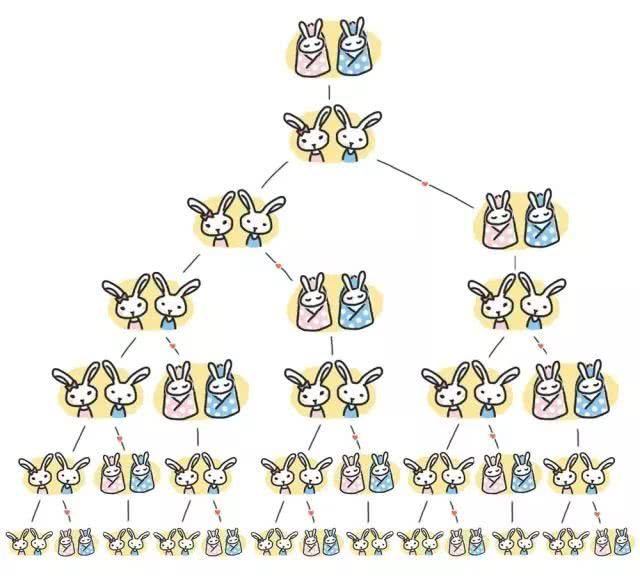
\includegraphics[scale=0.5]{img/Chapter3/3-2/1.png}
\end{figure}

\begin{lstlisting}[language=C++]
#include <iostream>

using namespace std;

int main()
{
    int n;
    cout << "Enter the number of terms: ";
    cin >> n;

    if(n == 1)
    {
        cout << "1" << endl;
    }
    else if(n == 2)
    {
        cout << "1, 1" << endl;
    }
    else
    {
        int num1, num2, val;
        num1 = 1;
        num2 = 1;
        cout << "1, 1";

        for(int i = 3; i <= n; i++)
        {
            val = num1 + num2;
            cout << ", " << val;
            num1 = num2;
            num2 = val;
        }
        cout << endl;
    }
    
    return 0;
}
\end{lstlisting}

\begin{tcolorbox}
    \mybox{运行结果}
    \begin{verbatim}
Enter the number of terms: 10
1, 1, 2, 3, 5, 8, 13, 21, 34, 55
\end{verbatim}
\end{tcolorbox}

\vspace{0.5cm}

\subsection{嵌套循环}

循环也可以嵌套使用,外层循环每执行一次,内层循环就会执行多次。

\vspace{-0.5cm}

\begin{lstlisting}[language=C++]
for(int i = 0; i < 2; i++)
{
    for(int j = 0; j < 3; j++)
    {
        cout << "i = " << i << ", j = " << j << endl;
    }
}
\end{lstlisting}

\begin{tcolorbox}
    \mybox{运行结果}
    \begin{verbatim}
i = 0, j = 0
i = 0, j = 1
i = 0, j = 2
i = 1, j = 0
i = 1, j = 1
i = 1, j = 2
\end{verbatim}
\end{tcolorbox}

\vspace{0.5cm}

\mybox{九九乘法表}\\

\begin{table}[H]
    \centering
    \setlength{\tabcolsep}{1.5mm}{
        \begin{tabular}{|c|c|c|c|c|c|c|c|c|}
            \hline
            1*1=1 & 1*2=2  & 1*3=3  & 1*4=4  & 1*5=5  & 1*6=6  & 1*7=7  & 1*8=8  & 1*9=9  \\
            \hline
            2*1=2 & 2*2=4  & 2*3=6  & 2*4=8  & 2*5=10 & 2*6=12 & 2*7=14 & 2*8=16 & 2*9=18 \\
            \hline
            3*1=3 & 3*2=6  & 3*3=9  & 3*4=12 & 3*5=15 & 3*6=18 & 3*7=21 & 3*8=24 & 3*9=27 \\
            \hline
            4*1=4 & 4*2=8  & 4*3=12 & 4*4=16 & 4*5=20 & 4*6=24 & 4*7=28 & 4*8=32 & 4*9=36 \\
            \hline
            5*1=5 & 5*2=10 & 5*3=15 & 5*4=20 & 5*5=25 & 5*6=30 & 5*7=35 & 5*8=40 & 5*9=45 \\
            \hline
            6*1=6 & 6*2=12 & 6*3=18 & 6*4=24 & 6*5=30 & 6*6=36 & 6*7=42 & 6*8=48 & 6*9=54 \\
            \hline
            7*1=7 & 7*2=14 & 7*3=21 & 7*4=28 & 7*5=35 & 7*6=42 & 7*7=49 & 7*8=56 & 7*9=63 \\
            \hline
            8*1=8 & 8*2=16 & 8*3=24 & 8*4=32 & 8*5=40 & 8*6=48 & 8*7=56 & 8*8=64 & 8*9=72 \\
            \hline
            9*1=9 & 9*2=18 & 9*3=27 & 9*4=36 & 9*5=45 & 9*6=54 & 9*7=63 & 9*8=72 & 9*9=81 \\
            \hline
        \end{tabular}
    }
\end{table}

\begin{lstlisting}[language=C++]
#include <iostream>

using namespace std;

int main()
{
    for(int i = 1; i <= 9; i++)
    {
        for(int j = 1; j <= 9; j++)
        {
            cout << i << "*" << j << "=" << i*j << "\t";
        }
        cout << endl;
    }
    return 0;
}
\end{lstlisting}

\vspace{0.5cm}

\mybox{打印图案}

\begin{lstlisting}
*
**
***
****
*****
\end{lstlisting}

\begin{lstlisting}[language=C++]
#include <iostream>

using namespace std;

int main()
{
    for(int i = 1; i <= 5; i++)
    {
        for(int j = 1; j <= i; j++)
        {
            cout << "*";
        }
        cout << endl;
    }
    return 0;
}
\end{lstlisting}

\newpage

\section{break or continue?}

\subsection{break}

break可用于跳出当前的switch或循环结构。在一些情况下,在循环的中途已经完成了某个目标,没有必要再进行剩余的循环,这时就可以使用break跳出循环。\\

例如在判断一个数$ n $是否为素数时,利用循环逐个判断$ 2 \sim n - 1 $之间的数是否能整除$ n $。只要发现其中有一个数能整除$ n $,就证明$ n $不是素数,可以跳出循环,不必再进行剩余的检查。\\

\mybox{素数}

\begin{lstlisting}[language=C++]
#include <iostream>
#include <cmath>

using namespace std;

int main()
{
    int n;
    cout << "Enter an integer: ";
    cin >> n;

    bool is_prime = true;
    for(int i = 2; i <= sqrt(n); i++)
    {
        if(n % i == 0)
        {
            is_prime = false;
            break;
        }
    }

    if(is_prime)
    {
        cout << n << " is a prime number" << endl;
    }
    else
    {
        cout << n << " is not a prime number" << endl;
    }

    return 0;
}
\end{lstlisting}

\begin{tcolorbox}
    \mybox{运行结果}
    \begin{verbatim}
Enter an integer: 17
17 is a prime number
\end{verbatim}
\end{tcolorbox}

\vspace{0.5cm}

\subsection{continue}

continue与break使用方法类似,但是它并不是跳出循环,而是跳过本轮循环,直接开始下一轮循环。\\

\mybox{正数平方和}

\begin{lstlisting}[language=C]
#include <iostream>

using namespace std;

int main()
{
    int n = 10;
    cout << "Enter " << n << " integers: ";

    int sum_square = 0;
    for(int i = 0; i < n; i++)
    {
        int num;
        cin >> num;
        if(num < 0)
        {
            continue;
        }

        sum_square += num * num;
    }

    cout << "Sum of squares of positive integers: "
            << sum_square << endl;
            
    return 0;
}
\end{lstlisting}

\begin{tcolorbox}
    \mybox{运行结果}
    \begin{verbatim}
Enter 10 integers: 5 7 -2 0 4 -4 -9 3 9 5
Sum of squares of positive integers: 205
\end{verbatim}
\end{tcolorbox}

\newpage